% Source PDF page 491 (printed p. 477)
\begin{figure}[htbp]\centering
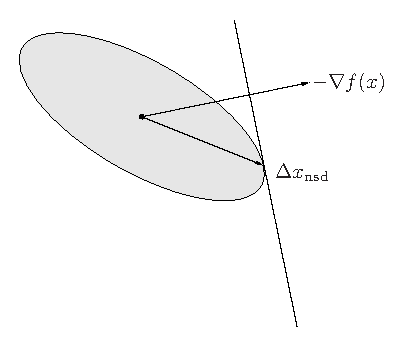
\includegraphics[width=.55\linewidth]{figures/ch09-fig09.pdf}
\caption*{图9.9\quad 二次范数的归一化最速下降方向。椭球是该范数的单位球，平移到点 $x$。$x$ 处的归一化最速下降方向 $\Delta x_{\mathrm{nsd}}$，在保持位于椭球内的同时，沿 $-\nabla f(x)$ 方向延伸尽可能远。图中表示了梯度方向和归一化最速下降方向。}
\end{figure}

\subsubsection*{通过坐标变换解释}
还可把最速下降方向 $\Delta x_{\mathrm{sd}}$ 解释为对问题进行坐标变换后的梯度搜索方向。定义 $\overline u=P^{1/2}u$，则 $\norm u_P=\norm{\overline u}_2$。利用此坐标变换，可通过最小化函数 $\overline f:\R^n\to\R$ 的等价问题，求解原来的 $f$ 最小化问题，其中
\[
\overline f(\overline u)=f(P^{-1/2}\overline u)=f(u).
\]
若对 $\overline f$ 应用梯度法，在 $\overline x$ 处（对应于原问题的 $x=P^{-1/2}\overline x$）的搜索方向为
\[
\Delta\overline x=-\nabla\overline f(\overline x)
=-P^{-1/2}\nabla f(P^{-1/2}\overline x)
=-P^{-1/2}\nabla f(x).
\]
这一梯度搜索方向对应于原变量 $x$ 的方向
\[
\Delta x=P^{-1/2}(-P^{-1/2}\nabla f(x))=-P^{-1}\nabla f(x).
\]
换言之，二次范数 $\norm{\cdot}_P$ 的最速下降法，可看作在坐标变换 $\overline x=P^{1/2}x$ 后对问题应用梯度法。

\subsection{\texorpdfstring{$\ell_1$}{ℓ₁} 范数下的最速下降}
再考虑 $\ell_1$ 范数的最速下降法。其归一化最速下降方向
\[
\Delta x_{\mathrm{nsd}}=\argmin\{\nabla f(x)^\T v\mid\norm v_1\le1\}
\]
容易刻画。

% Source PDF page 492 (printed p. 478)
\begin{figure}[htbp]\centering
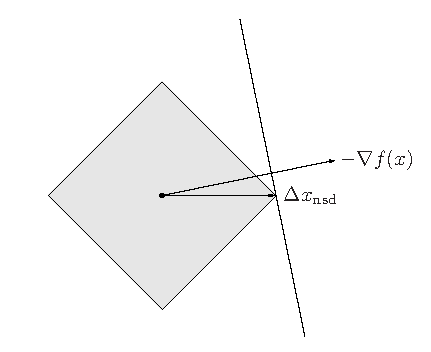
\includegraphics[width=.55\linewidth]{figures/ch09-fig10.pdf}
\caption*{图9.10\quad $\ell_1$ 范数的归一化最速下降方向。菱形为平移到 $x$ 的 $\ell_1$ 范数单位球。归一化最速下降方向总能取为某个标准基向量方向；本例中为 $\Delta x_{\mathrm{nsd}}=e_1$。}
\end{figure}
任取满足 $\norm{\nabla f(x)}_\infty=|(\nabla f(x))_i|$ 的指标 $i$，则一个 $\ell_1$ 范数归一化最速下降方向为
\[
\Delta x_{\mathrm{nsd}}
=-\operatorname{sign}\left(\frac{\partial f(x)}{\partial x_i}\right)e_i,
\]
其中 $e_i$ 是第 $i$ 个标准基向量。未归一化的最速下降步为
\[
\Delta x_{\mathrm{sd}}
=\Delta x_{\mathrm{nsd}}\norm{\nabla f(x)}_\infty
=-\frac{\partial f(x)}{\partial x_i}e_i.
\]
因此，$\ell_1$ 范数归一化最速下降步总可选为标准基向量或其相反数；它是使 $f$ 近似减小量最大的坐标轴方向，如图9.10所示。

$\ell_1$ 范数最速下降算法有很自然的解释：每次迭代选择 $\nabla f(x)$ 中绝对值最大的分量，再按 $(\nabla f(x))_i$ 的符号减小或增加 $x$ 的相应分量。由于每次迭代只更新 $x$ 的一个分量，它有时称为\emph{坐标下降算法}。这能大大简化线搜索，甚至使其变得极简单。

\begin{origexample}{9.2}
\emph{Frobenius范数缩放。}§4.5.4中遇到无约束几何规划
\[
\text{最小化}\quad\sum_{i,j=1}^n M_{ij}^2d_i^2/d_j^2,
\]
其中给定 $M\in\R^{n\times n}$，变量为 $d\in\R^n$。用变量替换 $x_i=2\log d_i$，可写为凸形式
\[
\text{最小化}\quad
f(x)=\log\left(\sum_{i,j=1}^n M_{ij}^2e^{x_i-x_j}\right).
\]

% Source PDF page 493 (printed p. 479)
每次仅对一个分量最小化 $f$ 很容易。保持除第 $k$ 个分量以外的所有分量不变，可写
$f(x)=\log(\alpha_k+\beta_ke^{-x_k}+\gamma_ke^{x_k})$，其中
\[
\alpha_k=M_{kk}^2+\sum_{i,j\ne k}M_{ij}^2e^{x_i-x_j},\quad
\beta_k=\sum_{i\ne k}M_{ik}^2e^{x_i},\quad
\gamma_k=\sum_{j\ne k}M_{kj}^2e^{-x_j}.
\]
$f(x)$ 作为 $x_k$ 的函数，在 $x_k=\log(\beta_k/\gamma_k)/2$ 处最小。因此，本例精确线搜索可用简单解析公式完成。

精确线搜索的 $\ell_1$ 最速下降算法重复以下步骤。
\begin{enumerate}
\item 计算梯度
\[
(\nabla f(x))_i=
\frac{-\beta_ie^{-x_i}+\gamma_ie^{x_i}}
{\alpha_i+\beta_ie^{-x_i}+\gamma_ie^{x_i}},\quad i=1,\ldots,n.
\]
\item 选择 $\nabla f(x)$ 的一个绝对值最大的分量：
$|\nabla f(x)|_k=\norm{\nabla f(x)}_\infty$。
\item 令 $x_k=\log(\beta_k/\gamma_k)/2$，在标量变量 $x_k$ 上最小化 $f$。
\end{enumerate}
\end{origexample}

\subsection{收敛分析}
本节将回溯线搜索梯度法的收敛分析推广到任意范数的最速下降法。利用任意范数可用欧几里得范数求界这一事实，即存在常数 $\gamma,\widetilde\gamma\in(0,1]$，满足
\[
\norm x\ge\gamma\norm x_2,\qquad
\norm x_*\ge\widetilde\gamma\norm x_2
\]
（见§A.1.4）。

仍假设 $f$ 在初始下水平集 $S$ 上强凸。上界 $\nabla^2f(x)\preceq MI$ 给出函数 $f(x+t\Delta x_{\mathrm{sd}})$ 关于 $t$ 的上界：
\begin{align}
f(x+t\Delta x_{\mathrm{sd}})
&\le f(x)+t\nabla f(x)^\T\Delta x_{\mathrm{sd}}
+\frac{M\norm{\Delta x_{\mathrm{sd}}}_2^2}{2}t^2\notag\\
&\le f(x)+t\nabla f(x)^\T\Delta x_{\mathrm{sd}}
+\frac{M\norm{\Delta x_{\mathrm{sd}}}^2}{2\gamma^2}t^2\notag\\
&=f(x)-t\norm{\nabla f(x)}_*^2
+\frac{M}{2\gamma^2}t^2\norm{\nabla f(x)}_*^2.\tag{9.26}
\end{align}
使二次上界（9.26）最小的步长 $\widehat t=\gamma^2/M$ 满足回溯线搜索退出条件：
\begin{equation}
\begin{split}
f(x+\widehat t\Delta x_{\mathrm{sd}})
&\le f(x)-\frac{\gamma^2}{2M}\norm{\nabla f(x)}_*^2\\
&\le f(x)+\frac{\alpha\gamma^2}{M}\nabla f(x)^\T\Delta x_{\mathrm{sd}},
\end{split}\tag{9.27}
\end{equation}

% Source PDF page 494 (printed p. 480)
因为 $\alpha<1/2$ 且 $\nabla f(x)^\T\Delta x_{\mathrm{sd}}=-\norm{\nabla f(x)}_*^2$。因此，线搜索返回步长 $t\ge\min\{1,\beta\gamma^2/M\}$，从而
\[
\begin{aligned}
f(x^+)=f(x+t\Delta x_{\mathrm{sd}})
&\le f(x)-\alpha\min\{1,\beta\gamma^2/M\}\norm{\nabla f(x)}_*^2\\
&\le f(x)-\alpha\widetilde\gamma^2\min\{1,\beta\gamma^2/M\}
\norm{\nabla f(x)}_2^2.
\end{aligned}
\]
两边减 $p^\star$，再用（9.9），得到
\[
f(x^+)-p^\star\le c(f(x)-p^\star),
\]
其中
\[
c=1-2m\alpha\widetilde\gamma^2\min\{1,\beta\gamma^2/M\}<1.
\]
因此
\[
f(x^{(k)})-p^\star\le c^k(f(x^{(0)})-p^\star),
\]
即与梯度法一样线性收敛。

\subsection{讨论与例子}
\subsubsection*{最速下降范数的选择}
定义最速下降方向所用范数的选择，可能极大影响收敛速率。为简便，考虑二次 $P$ 范数。§9.4.1已说明，它的最速下降法等同于在坐标变换 $\overline x=P^{1/2}x$ 后对问题应用梯度法。梯度法在下水平集（或最优点附近Hessian）条件数适中时效果好，条件数大时效果差。因此，坐标变换后下水平集条件适中，最速下降法就效果好。

这给出选择 $P$ 的原则：使经 $P^{-1/2}$ 变换后的 $f$ 下水平集条件良好。例如，若知道最优点处Hessian $H(x^\star)$ 的近似 $\widehat H$，一个很好的选择是 $P=\widehat H$，因为此时 $\widetilde f$ 在最优点处的Hessian为
\[
\widehat H^{-1/2}\nabla^2f(x^\star)\widehat H^{-1/2}\approx I,
\]
因而很可能有小条件数。

同一思想也可不用坐标变换表述。说下水平集经过 $\overline x=P^{1/2}x$ 变换后条件数小，等价于说椭球
\[
\mathcal E=\{x\mid x^\T Px\le1\}
\]
近似下水平集的形状。（即适当缩放和平移后，可很好地近似。）

收敛速率对 $P$ 选择的这种依赖，可从两面看。乐观的观点是，对于任意问题，总存在某种 $P$ 的选择，使最速下降法非常有效。

% Source PDF page 495 (printed p. 481)
\begin{figure}[htbp]\centering
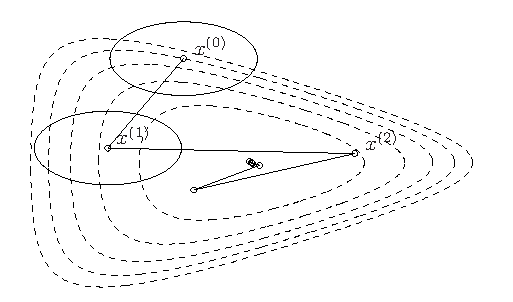
\includegraphics[width=.65\linewidth]{figures/ch09-fig11.pdf}
\caption*{图9.11\quad 采用二次范数 $\norm{\cdot}_{P_1}$ 的最速下降法。椭圆为 $x^{(0)}$ 和 $x^{(1)}$ 处范数球 $\{x\mid\norm{x-x^{(k)}}_{P_1}\le1\}$ 的边界。}
\end{figure}
难点当然是找到这样的 $P$。悲观的观点则是，对于任意问题，有大量 $P$ 的选择使最速下降法效果很差。总之，在能识别某个矩阵 $P$、使变换后问题的条件数适中的情况下，最速下降法效果好。

\subsubsection*{例子}
用目标为（9.20）的 $\R^2$ 非二次问题说明上述思想。采用两个二次范数的最速下降法，范数由
\[
P_1=\begin{bmatrix}2&0\\0&8\end{bmatrix},\qquad
P_2=\begin{bmatrix}8&0\\0&2\end{bmatrix}
\]
定义。两者都使用 $\alpha=0.1,\beta=0.7$ 的回溯线搜索。

图9.11、9.12显示 $\norm{\cdot}_{P_1}$ 和 $\norm{\cdot}_{P_2}$ 最速下降法的迭代点，图9.13显示两者误差随迭代次数的变化。范数选择强烈影响收敛：$\norm{\cdot}_{P_1}$ 比梯度法稍快，$\norm{\cdot}_{P_2}$ 则慢得多。

可通过分别经过 $\overline x=P_1^{1/2}x$ 和 $\overline x=P_2^{1/2}x$ 变换后的问题解释。图9.14、9.15显示变换坐标后的问题。$P_1$ 对应的变量替换得到条件数适中的下水平集，因而收敛快；$P_2$ 对应替换使下水平集条件更差，因而收敛较慢。

% Source PDF page 496 (printed p. 482)
\begin{figure}[htbp]\centering
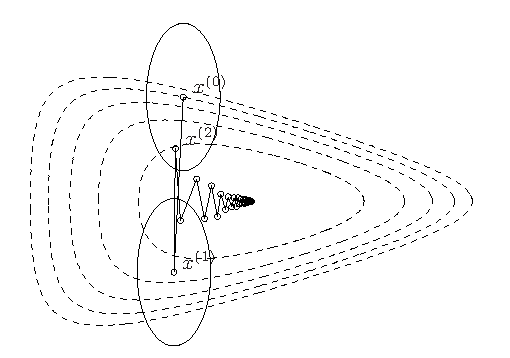
\includegraphics[width=.65\linewidth]{figures/ch09-fig12.pdf}
\caption*{图9.12\quad 采用二次范数 $\norm{\cdot}_{P_2}$ 的最速下降法。}
\end{figure}
\begin{figure}[htbp]\centering
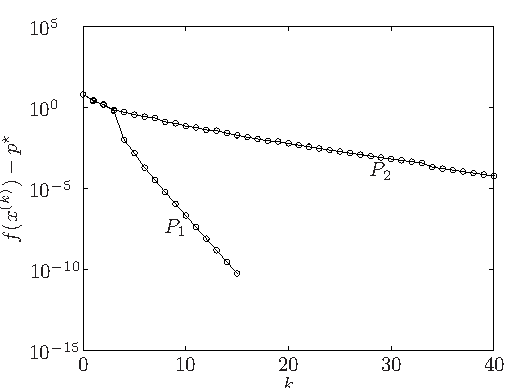
\includegraphics[width=.65\linewidth]{figures/ch09-fig13.pdf}
\caption*{图9.13\quad 采用二次范数 $\norm{\cdot}_{P_1}$ 和 $\norm{\cdot}_{P_2}$ 的最速下降法误差 $f(x^{(k)})-p^\star$ 随迭代次数 $k$ 的变化。$\norm{\cdot}_{P_1}$ 收敛快，$\norm{\cdot}_{P_2}$ 收敛很慢。}
\end{figure}

% Source PDF page 497 (printed p. 483)
\begin{figure}[htbp]\centering
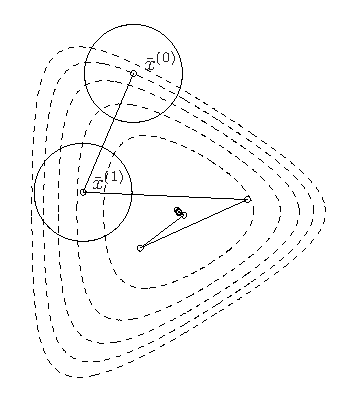
\includegraphics[width=.5\linewidth]{figures/ch09-fig14.pdf}
\caption*{图9.14\quad 坐标变换后，范数 $\norm{\cdot}_{P_1}$ 最速下降法的迭代点。这一变换减小下水平集条件数，从而加快收敛。}
\end{figure}
\begin{figure}[htbp]\centering
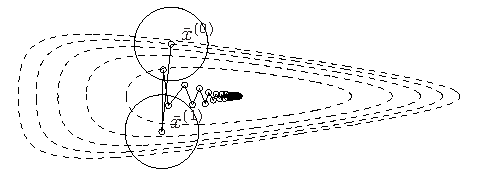
\includegraphics[width=.65\linewidth]{figures/ch09-fig15.pdf}
\caption*{图9.15\quad 坐标变换后，范数 $\norm{\cdot}_{P_2}$ 最速下降法的迭代点。这一变换增大下水平集条件数，从而减慢收敛。}
\end{figure}

% Source PDF page 498 (printed p. 484)
\begin{figure}[htbp]\centering
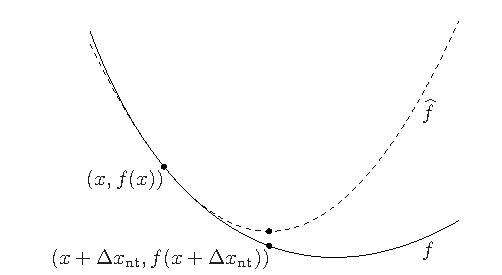
\includegraphics[width=.65\linewidth]{figures/ch09-fig16.pdf}
\caption*{图9.16\quad 函数 $f$（实线）与它在 $x$ 处的二阶近似 $\widehat f$（虚线）。将牛顿步 $\Delta x_{\mathrm{nt}}$ 加到 $x$ 上，就得到 $\widehat f$ 的最小点。}
\end{figure}
\section{牛顿法}
\subsection{牛顿步}
对 $x\in\dom f$，向量
\[
\Delta x_{\mathrm{nt}}=-\nabla^2f(x)^{-1}\nabla f(x)
\]
称为（$f$ 在 $x$ 处的）\emph{牛顿步}。$\nabla^2f(x)$ 的正定性意味着，除非 $\nabla f(x)=0$，否则
\[
\nabla f(x)^\T\Delta x_{\mathrm{nt}}
=-\nabla f(x)^\T\nabla^2f(x)^{-1}\nabla f(x)<0.
\]
因此牛顿步是下降方向（除非 $x$ 最优）。可以从几种角度解释并说明牛顿步。

\subsubsection*{二阶近似的最小点}
$f$ 在 $x$ 处的二阶Taylor近似（或模型）$\widehat f$ 为
\begin{equation}
\widehat f(x+v)=f(x)+\nabla f(x)^\T v+\tfrac12v^\T\nabla^2f(x)v.\tag{9.28}
\end{equation}
它是关于 $v$ 的凸二次函数，在 $v=\Delta x_{\mathrm{nt}}$ 时最小。因此，在 $x$ 上加牛顿步 $\Delta x_{\mathrm{nt}}$，就使 $f$ 在 $x$ 的二阶近似最小，如图9.16所示。

这个解释有助于理解牛顿步。若 $f$ 是二次函数，则 $x+\Delta x_{\mathrm{nt}}$ 就是精确最小点。若 $f$ 近似二次，直觉表明 $x+\Delta x_{\mathrm{nt}}$ 应很好地估计 $f$ 的最小点 $x^\star$。由于 $f$ 二阶可微，$x$ 靠近 $x^\star$ 时，其二次模型会很准确。因此 $x$ 靠近 $x^\star$ 时，$x+\Delta x_{\mathrm{nt}}$ 应很好地估计 $x^\star$。将会看到，这一直觉是正确的。

% Source PDF page 499 (printed p. 485)
\begin{figure}[htbp]\centering
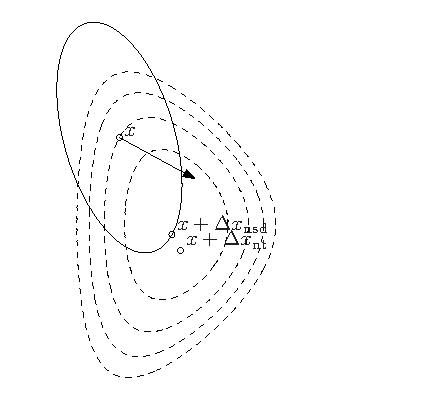
\includegraphics[width=.55\linewidth]{figures/ch09-fig17.pdf}
\caption*{图9.17\quad 虚线为凸函数的等值线，实线椭球为 $\{x+v\mid v^\T\nabla^2f(x)v\le1\}$。箭头表示梯度下降方向 $-\nabla f(x)$。牛顿步 $\Delta x_{\mathrm{nt}}$ 是范数 $\norm{\cdot}_{\nabla^2f(x)}$ 的最速下降方向；图中还表示该范数的归一化最速下降方向 $\Delta x_{\mathrm{nsd}}$。}
\end{figure}
\subsubsection*{Hessian范数下的最速下降方向}
牛顿步也是Hessian $\nabla^2f(x)$ 定义的二次范数
\[
\norm u_{\nabla^2f(x)}=(u^\T\nabla^2f(x)u)^{1/2}
\]
在 $x$ 处的最速下降方向。这再次说明为何牛顿步应是好的搜索方向，且 $x$ 靠近 $x^\star$ 时尤其好。

回顾上文讨论，若坐标变换后Hessian条件数小，二次范数 $\norm{\cdot}_P$ 最速下降法就收敛很快。特别地，在 $x^\star$ 附近，$P=\nabla^2f(x^\star)$ 是很好的选择。当 $x$ 靠近 $x^\star$，有 $\nabla^2f(x)\approx\nabla^2f(x^\star)$，由此解释牛顿步为何是极好的搜索方向，如图9.17所示。

\subsubsection*{线性化最优性条件的解}
在 $x$ 附近线性化最优性条件 $\nabla f(x^\star)=0$，得到
\[
\nabla f(x+v)\approx\nabla f(x)+\nabla^2f(x)v=0,
\]
这是关于 $v$ 的线性方程，解为 $v=\Delta x_{\mathrm{nt}}$。因此，在 $x$ 上加牛顿步就使线性化最优性条件成立。这同样表明，$x$ 靠近 $x^\star$（最优性条件已接近成立）时，更新 $x+\Delta x_{\mathrm{nt}}$ 应很好地近似 $x^\star$。

当 $n=1$，即 $f:\R\to\R$ 时，解释尤其简单。最小化问题的解 $x^\star$ 由 $f'(x^\star)=0$ 刻画，即导数 $f'$ 的过零点。

% Source PDF page 500 (printed p. 486)
\begin{figure}[htbp]\centering
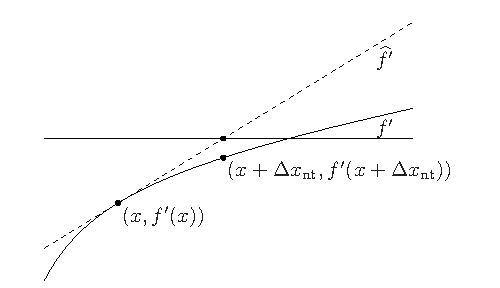
\includegraphics[width=.65\linewidth]{figures/ch09-fig18.pdf}
\caption*{图9.18\quad 实线为图9.16中 $f$ 的导数 $f'$。$\widehat f'$ 是 $f'$ 在 $x$ 处的线性近似。牛顿步 $\Delta x_{\mathrm{nt}}$ 是 $\widehat f'$ 的根与点 $x$ 的差。}
\end{figure}
由于 $f$ 凸，$f'$ 单调递增。给定当前解的近似 $x$，在 $x$ 处对 $f'$ 作一阶Taylor近似，这个仿射近似的过零点就是 $x+\Delta x_{\mathrm{nt}}$，如图9.18所示。

\subsubsection*{牛顿步的仿射不变性}
牛顿步的重要特点是独立于线性或仿射坐标变换。设 $T\in\R^{n\times n}$ 非奇异，定义 $\overline f(y)=f(Ty)$。有
\[
\nabla\overline f(y)=T^\T\nabla f(x),\qquad
\nabla^2\overline f(y)=T^\T\nabla^2f(x)T,
\]
其中 $x=Ty$。因此，$\overline f$ 在 $y$ 处的牛顿步为
\[
\begin{aligned}
\Delta y_{\mathrm{nt}}
&=-\bigl(T^\T\nabla^2f(x)T\bigr)^{-1}T^\T\nabla f(x)\\
&=-T^{-1}\nabla^2f(x)^{-1}\nabla f(x)\\
&=T^{-1}\Delta x_{\mathrm{nt}},
\end{aligned}
\]
其中 $\Delta x_{\mathrm{nt}}$ 是 $f$ 在 $x$ 处的牛顿步。因此 $f$ 和 $\overline f$ 的牛顿步由同一线性变换联系，并且
\[
x+\Delta x_{\mathrm{nt}}=T(y+\Delta y_{\mathrm{nt}}).
\]

\subsubsection*{牛顿减量}
量
\[
\lambda(x)=\bigl(\nabla f(x)^\T\nabla^2f(x)^{-1}\nabla f(x)\bigr)^{1/2}
\]
称为 $x$ 处的\emph{牛顿减量}。将会看到，它在牛顿法分析中起重要作用，也可用于
